% This textfile includes
% 3. Analysis procedures
%    ..
%    ..
%    3.9 Systematic uncertainties

\section{Systematic uncertainties}
The background and signal predictions are affected by systematic uncertainties that have to be estimated and taken into account for limit setting. This section includes a list of the relevant systematic uncertainties for this analysis and how they are estimated.

\begin{itemize}
\item \textbf{Luminosity:} The overall uncertainty of the LHC luminosity delivered to CMS in the 2012 Run-I is measured to be 2.6\%\cite{lumi}
\item \textbf{Jet energy scale:} The systematic on the jet energy scale was studied by scaling up and down the jet mass and $p_{T}$ according to the uncertainty associated to the jet energy corrections used. The Zh mass distributions reconstructed by jet four-momentum is affected and therefore we consider the shape uncertainty as well, shown in Fig.~\ref{fig:SYS_JES}. The overall uncertainty is about 8\%.
\item \textbf{CSV distribution normalization:} This systematic is from normalizing the CSV distributions of MC background prediction in order to fit the data, it is estimated about 10\% for each background.
\item \textbf{Pile-up reweighting:} As described previously in section 3.4, we reweight the pile-up interactions in MC predictions for better modeling. To calculate the uncertainties on the pile-up simulation, we produce two pile-up distributions where the minimum bias cross section is shifted by $\pm$5\%\cite{PileupError}. The impact on the event yields is about 2\%. Despite the effects are small, we still consider shape uncertainties of pile-up. Fig.~\ref{fig:SYS_PU} shows the variation distributions of number of vertices for $\pm1\sigma$.
\item \textbf{Lepton ID scale factor:} Text.
\end{itemize}

\begin{figure}[hbtp]
  \centering
  \subfigure[The systematic uncertainty of jet energy scale on background MC $m_{Zh}$ spectrum.]{
    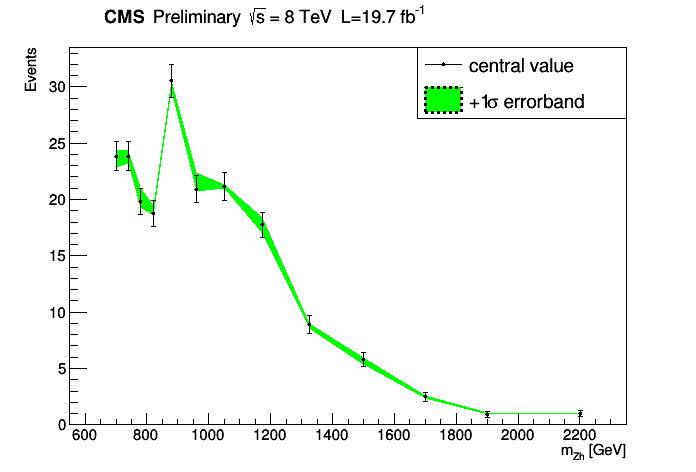
\includegraphics[scale=0.28]{figure/CH3/Systematics/Bkg_jes.png}}
  \hspace{0.5cm}
  \subfigure[The systematic uncertainty of jet energy scale on signal MC $m_{Zh}$ spectrum.]{
    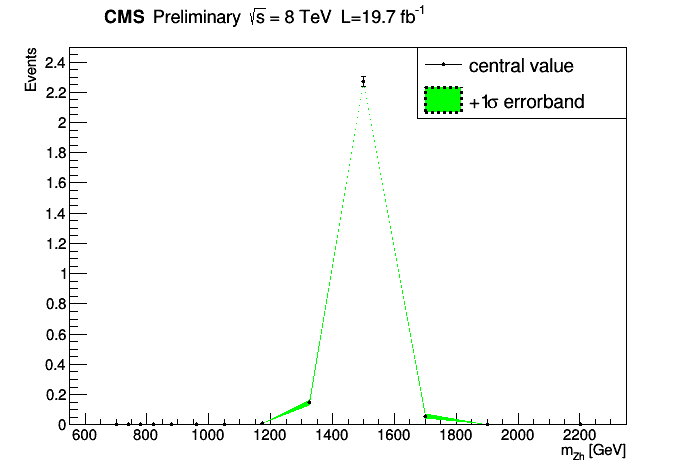
\includegraphics[scale=0.28]{figure/CH3/Systematics/Sig_jes.png}}
  \caption{\label{fig:SYS_JES}SR $m_{Zh}$ distributions for both signal (1500 GeV) and background MC samples. The uncertainty of jet energy scale is shown as the green error band ($\pm1 \sigma$), while the error bar presents the statistic error.}
\end{figure}

\begin{figure}[hbtp]
  \centering
  \subfigure[Number of vertices in electron channel.]{
    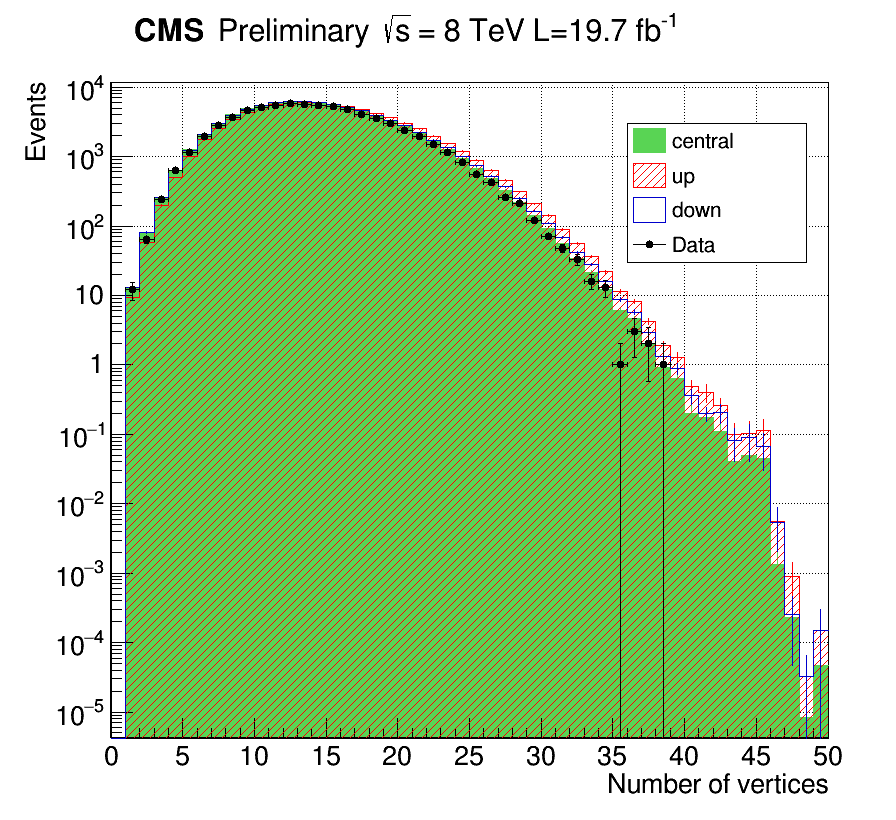
\includegraphics[scale=0.22]{figure/CH3/Systematics/h_nVtx_El_SysLog.png}}
  \hspace{0.5cm}
  \subfigure[Number of vertices in muon channel.]{
    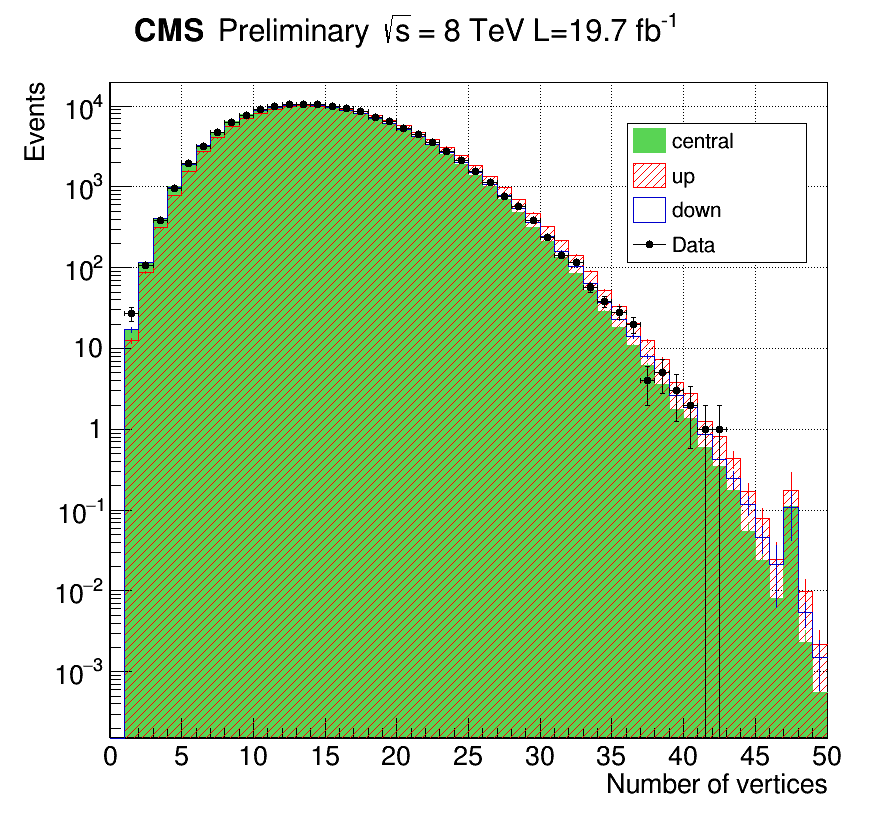
\includegraphics[scale=0.22]{figure/CH3/Systematics/h_nVtx_Mu_SysLog.png}}
  \caption{\label{fig:SYS_PU}(a) shows the distributions of number of vertices in electron channel, comparing central value of the total background prediction and the $\pm1\sigma$ variation, and data as well. (b) shows the result in muon channel.}
\end{figure}
